\section{M�lemetode og Instrumentering}

En av utfordningene er � f� til et laboppsett som kan m�le og karakterisere ulike former for tap, slik som dislokasjonslinjer, forurensninger, og korngrenser. Dette er viktig for � kunne forst� �rsakene til tap, og for � kunne analysere hvilke framstillingsprosesser som gir et gunstig resultat.

\begin{figure}%
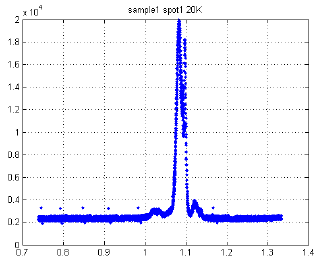
\includegraphics[width=\columnwidth]{bilder/cryolabtap.png}%
\caption{Fotoluminisensspekter ved 20K i cryolab}%
\label{fig:cryolabtap}%
\end{figure}

Publikasjoner som ~\cite{tarasov00} (figur \ref{fig:dislokasjonslinjer}) viser et tapsspekter rundt 0,7-1 eV som ikke er synlig p� m�linger gjort p� cryolab. (figur \ref(fig:cryolabtap)) Grunnen til det er ikke kjent, men antas og v�re et resultat av tap i utstyr som linser og beamsplittere. 

1eV tilsvarer 1240nm b�lgelengde fra ~\ref(lysenergi), som betyr at spekteret som antas � forsvinne har b�lgelengde 1100-1700nm.



%Hvordan l�se problemet?

%Utstyret som er p� labben er spesifisert til � v�re tiln�rmet tapsfritt for b�lgelengder 630-1000nm, mens alt over 1000nm ser ut til � %forsvinne i oppsettet. 
